% gm-08-Radians.tex

\documentclass[xcolor=dvipsnames]{beamer}

\usepackage{cancel}
\renewcommand{\CancelColor}{\color{red}}
\usepackage{graphicx}
\usepackage{wrapfig}
\usepackage{colortbl}
\usepackage{color}
\usepackage{alltt}
\renewcommand*{\thefootnote}{\fnsymbol{footnote}}
\definecolor{myblue}{rgb}{0.8,0.85,1}

\mode<presentation>
{
  \usetheme{Warsaw}
  \setbeamercovered{transparent}
}
% \usecolortheme[named=OliveGreen]{structure}
\setbeamertemplate{navigation symbols}{} 
\setbeamertemplate{blocks}[rounded][shadow=true] 

% this is for overlaying math symbols, see https://tex.stackexchange.com/questions/12895/overlay-symbol-with-another
\def\qeq{\mathrel{%
    \mathchoice{\QEQ}{\QEQ}{\scriptsize\QEQ}{\tiny\QEQ}%
}}
\def\QEQ{{%
    \setbox0\hbox{$\longrightarrow$}%
    \rlap{\hbox to \wd0{\hss/\hss}}\box0
  }}

\newcounter{expls}
\setcounter{expls}{0}
\newcommand{\beispiel}[1]{\refstepcounter{expls}\textbf{Example \arabic{expls}: #1.}}

\newcounter{exercise}
\setcounter{exercise}{0}
\newcommand{\ubung}[0]{\refstepcounter{exercise}\textbf{Exercise \arabic{exercise}: }}

\newif\ifBCITCourse
\BCITCoursetrue
% \BCITCoursefalse
\newif\ifWhichCourse
\WhichCoursetrue
\WhichCoursefalse
\ifBCITCourse
\ifWhichCourse
\newcommand{\CourseName}{Technical Mathematics for Food Technology}
\newcommand{\CourseNumber}{MATH 1441}
\newcommand{\CourseInst}{BCIT}
\else
\newcommand{\CourseName}{Technical Mathematics for Geomatics}
\newcommand{\CourseNumber}{MATH 1511}
\newcommand{\CourseInst}{BCIT}
\fi
\else
\newcommand{\CourseName}{Philosophy and Literature}
\newcommand{\CourseNumber}{PHIL 375}
\newcommand{\CourseInst}{UBC}
\fi

\title{Radians}
\subtitle{{\CourseNumber}, BCIT}

\author{\CourseName}

\date{October 11, 2017}

\begin{document}

\begin{frame}
  \titlepage
\end{frame}

\begin{frame}
  \frametitle{Whole Circle Bearing}
  Let there be two points $A$ and $B$. The \alert{whole circle
    bearing} from $A$ to $B$ is the angle by which a straight line
  from $A$ to $B$ deviates clockwise from a line going straight North
  at $A$. Here is an example. 
  \begin{itemize}
  \item Consider points $P=(-177.264,-344.223)$ and
  $Q=(455.761,225.099)$ in the plane. All units are metres. What is
  the whole circle bearing from $P\rightarrow{}Q$, and what is the
  whole circle bearing from $Q\rightarrow{}P$?
  \end{itemize}
\end{frame}

\begin{frame}
  \frametitle{Whole Circle Bearing Diagram}
  \begin{figure}[h]
    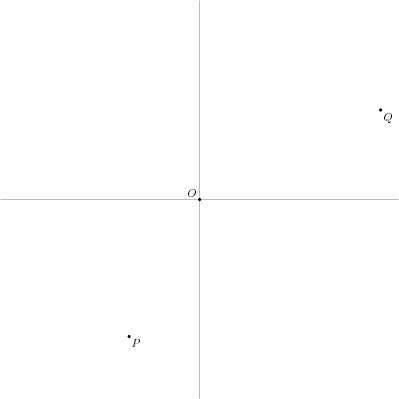
\includegraphics[scale=.6]{./wcbc.png}
  \end{figure}
\end{frame}

\begin{frame}
  \frametitle{Whole Circle Bearing Diagram}
  \begin{figure}[h]
    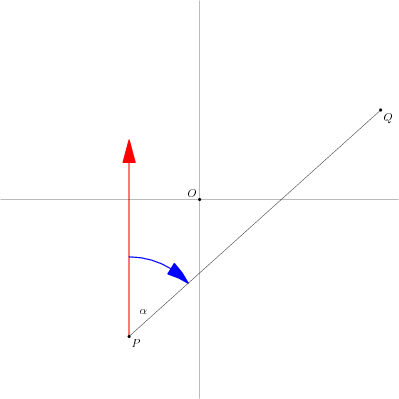
\includegraphics[scale=.6]{./wcbb.png}
  \end{figure}
\end{frame}

\begin{frame}
  \frametitle{Whole Circle Bearing Diagram}
  \begin{figure}[h]
    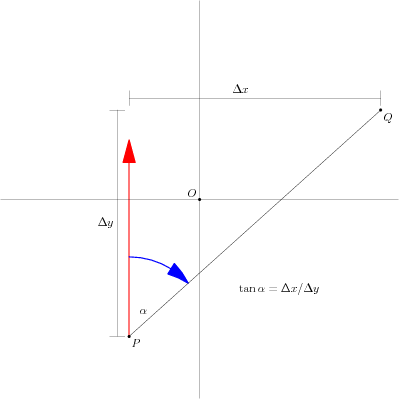
\includegraphics[scale=.6]{./wcba.png}
  \end{figure}
\end{frame}

\begin{frame}
  \frametitle{Whole Circle Bearing Diagram}
  \begin{figure}[h]
    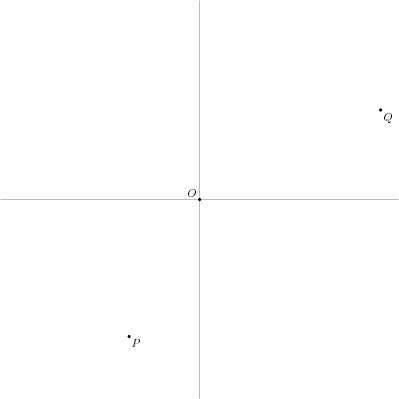
\includegraphics[scale=.6]{./wcbc.png}
  \end{figure}
\end{frame}

\begin{frame}
  \frametitle{Whole Circle Bearing Diagram}
  \begin{figure}[h]
    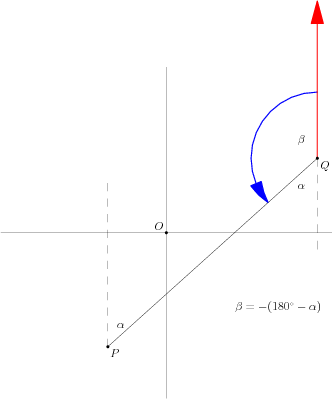
\includegraphics[scale=.6]{./wcca.png}
  \end{figure}
\end{frame}

\begin{frame}
  \frametitle{Radians}
What kind of animal is $30^{\circ}$? It is a real number -- not the
one you might expect. Just as $25\%$ is not the number 25, but the
number $0.25$; $30^{\circ}$ is not the number 30, but the number
$\pi/6$. The \mbox{symbol $^{\circ}$} (pronounced ``degrees'') is equivalent
to the factor $\pi/180$; just as the symbol $\%$ (pronounced
``percent'') is equivalent to the factor $1/100$. 
  \begin{figure}[h]
    
\includegraphics[scale=.5]{./degreeradians.jpg}
  \end{figure}
\end{frame}

\begin{frame}
  \frametitle{Radians Exercise}
{\ubung} A section of land is a wedge shape as shown. Calculate the perimeter
of the property.
  \begin{figure}[h]
    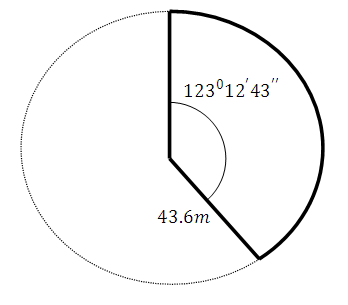
\includegraphics[scale=.5]{./radians.png}
  \end{figure}
\end{frame}

\begin{frame}
  \frametitle{Radians Exercise}
{\ubung} Consider the portion of a circular road curve shown.
\begin{enumerate}
\item What is the central angle?
\item What is the length of the outside curve of the road?
\end{enumerate}
  \begin{figure}[h]
    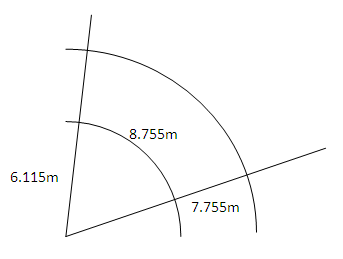
\includegraphics[scale=.5]{./radianz.png}
  \end{figure}
\end{frame}

\begin{frame}
  \frametitle{Latitude and Longitude}
Suppose that the surface of the earth can be
modeled on a perfect sphere with a radius of
$6378.1km$.

Let the coordinate of a point $P$ on the surface
of the earth be defined by its
\begin{enumerate}
\item longitude $\lambda$
\item latitude $\varphi$
\end{enumerate}
\begin{figure}[h]
    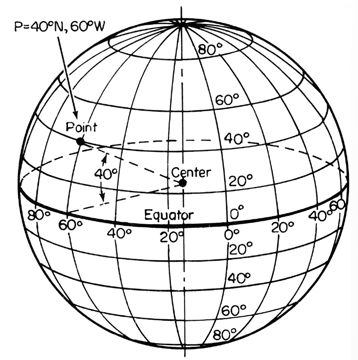
\includegraphics[scale=.5]{./latlong.png}
  \end{figure}
\end{frame}

\begin{frame}
  \frametitle{Latitude and Longitude Exercises}
\begin{enumerate}
\item<1-> Calculate the distance from the equator to the North Pole.
\item<2-> Calculate the distance from the North Pole to the South
  Pole.
\item<3-> How many kilometers north of the equator is a town of
  latitude $\varphi=43^{\circ}$?
\item<4-> How far apart, following along a line of longitude, are the two
  towns Brandon, Manitoba ($50^{\circ}N,100^{\circ}W$) and Dodge City, Kansas
  ($38^{\circ}N,100^{\circ}W$)?
\item<5-> A plane travels along the equator from $23^{\circ}E$ to $28^{\circ}E$.
  Calculate the distance travelled by the plane.
\end{enumerate}
\end{frame}

\begin{frame}
  \frametitle{Latitude and Longitude Exercises}
\begin{enumerate}
\item<1-> A plane travels along the equator from $23^{\circ}E$ to
  $128^{\circ}W$. Calculate the distance travelled by the plane.
\item<2-> What is the radius of the circle of constant latitude
  $\varphi=18^{\circ}N$?
\item<3-> Consider two towns, Windsor, Nova Scotia, at
  ($45^{\circ}N,65^{\circ}W$) and Grenoble, France at
  ($45^{\circ}N,5^{\circ}E$). If you follow a line of latitude, how
  far are the two towns apart?
\end{enumerate}
\end{frame}

\begin{frame}
  \frametitle{Distance Along a Great Circle}
  Let $R=6378.1$ be the radius of the Earth. Furthermore, let
  \begin{equation}
    \label{eq:ohheibif}
    \mbox{haversin}{}x=\sin^{2}\left(\frac{x}{2}\right)
  \end{equation}
  Then the great circle distance $d$ between two points $P_{1}$ and
  $P_{2}$ with latitudes $\varphi_{1},\varphi_{2}$ and longitudes
  $\lambda_{1},\lambda_{2}$ respectively is
  \begin{equation}
    \label{eq:ohpishah}
    \mbox{haversin}\left(\frac{d}{R}\right)=\mbox{haversin}(\varphi_{2}-\varphi_{1})+\cos\varphi_{1}\cos\varphi_{2}\mbox{haversin}(\lambda_{2}-\lambda_{1})\notag
  \end{equation}
  Use this formula to calculate the great circle distance between
  Windsor, Nova Scotia, and Grenoble, France. You may want to check
  your work using an online great circle distance calculator:
  \begin{center}
    \texttt{http://rifkin.com/1-waypoint/gps1-calc.html}
  \end{center}
\end{frame}

\begin{frame}
  \frametitle{Distance Along a Great Circle}
  Consider the two cities Krakow in Poland (50$^{\circ}$N,
  20$^{\circ}$E) and Campbell River on Vancouver Island
  (50$^{\circ}$N, 125$^{\circ}$W). Compare how far apart they are
  along a latitudinal circle (which is what ships would have followed
  if they had used the ``westing'' method) and along a great circle.
\end{frame}

\begin{frame}
  \frametitle{Polaris and Latitude}
  What is the latitude of a point at which Polaris is viewed as in the
  diagram with angle $\vartheta$?
    \begin{figure}[h]
    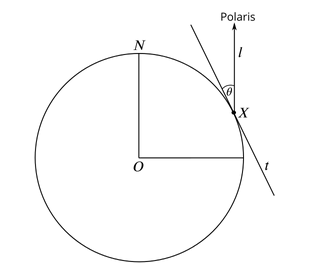
\includegraphics[scale=.5]{./polaris.png}
  \end{figure}
\end{frame}

\begin{frame}
  \frametitle{Exercises Oblique Triangles 1}
  A fir tree stands upright on a mountainside which rises uniformly at
  an angle of $16^{\circ}20'$. The tree breaks at a point 30 feet from
  the ground, the top striking down the slope of the mountain 26 feet
  from the foot of the tree. How high was the tree before it broke?
\end{frame}

\begin{frame}
  \frametitle{Exercises Oblique Triangles 1 Diagram}
    \begin{figure}[h]
    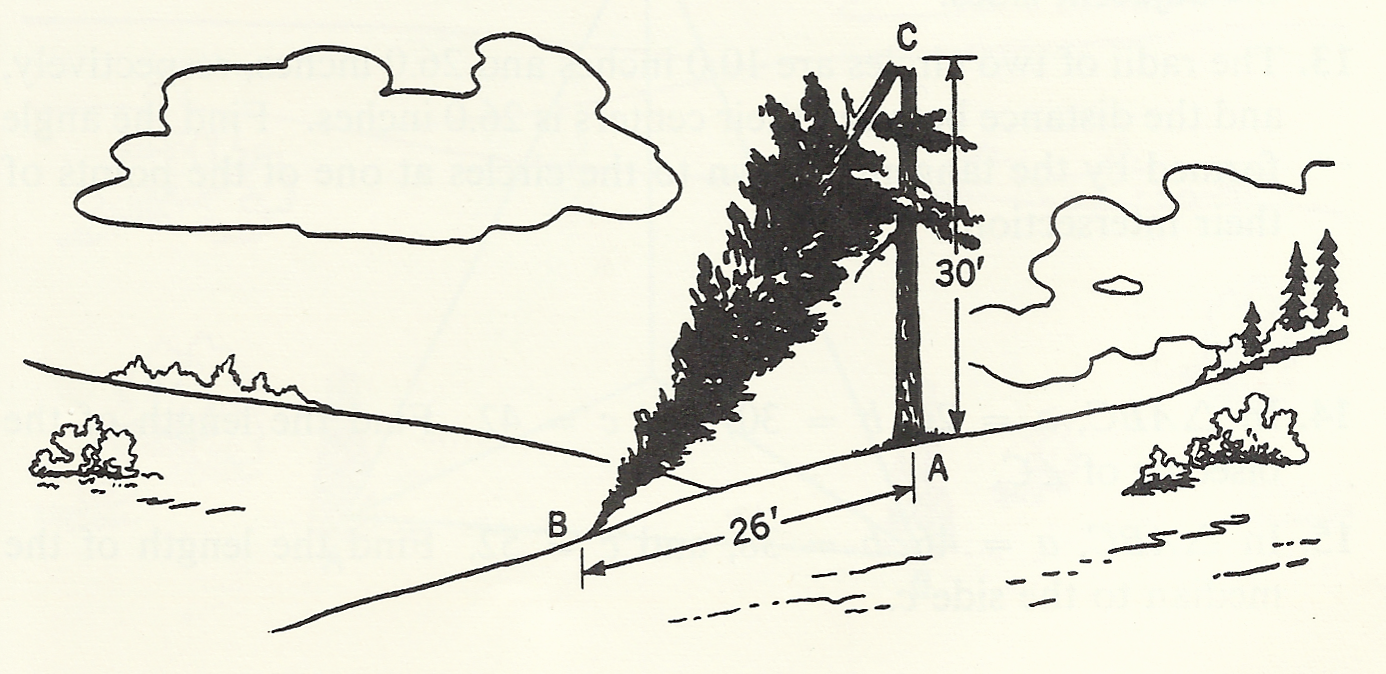
\includegraphics[scale=1]{./oblique-01.png}
  \end{figure}
\end{frame}

\begin{frame}
  \frametitle{Exercises Oblique Triangles 2}
The bearing of a ship at $C$ was north from $A$ and N $61^{\circ}$ W from $B$.
Later when the ship was at $D$, its bearing was N $53^{\circ}$ E from $A$ and
N $10^{\circ}$ W from $B$. If $A$ and $B$ are 6200 feet apart and $B$ is directly
east of $A$, how far apart are $C$ and $D$?
\end{frame}

\begin{frame}
  \frametitle{Exercises Oblique Triangles 2 Diagram}
    \begin{figure}[h]
    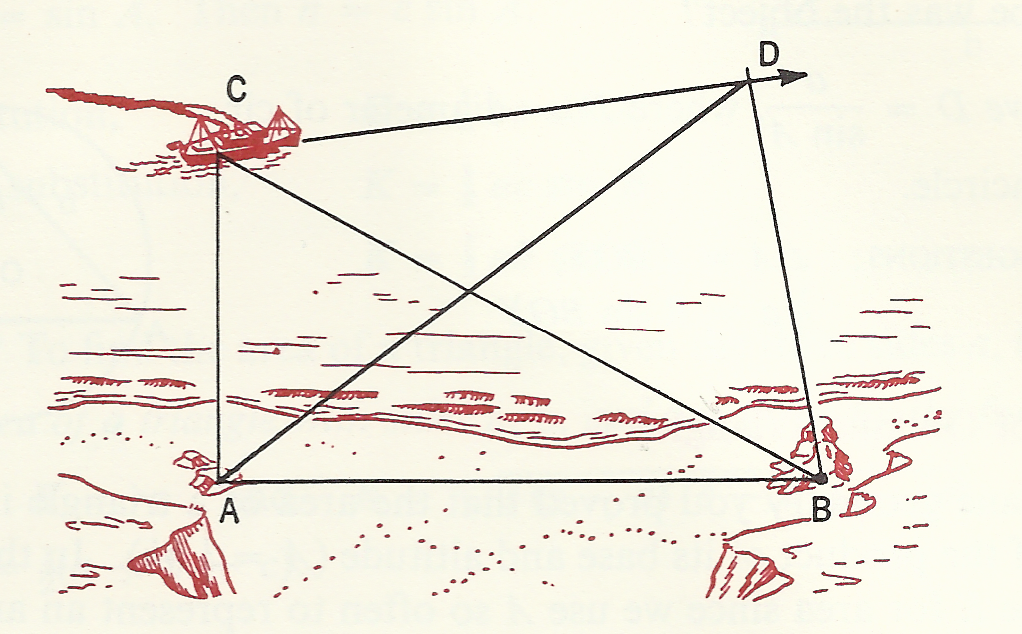
\includegraphics[scale=1]{./oblique-02.png}
  \end{figure}
\end{frame}

\begin{frame}
  \frametitle{Exercises Oblique Triangles 3}
  From two stations, $A$ and $B$, 4800 feet apart on level ground,
  observations were made on a stationary balloon. From $A$ the angle
  of elevation of the balloon was $42^{\circ}34'$. The angle formed by
  the vertical plane through $A$ and $P$ and the vertical plane
  through $A$ and $B$ was $20^{\circ}42'$. The angle formed by the
  vertical plane through $B$ and $P$ and the vertical plane through
  $B$ and $A$ was $35^{\circ}10'$. How high was the balloon?
\end{frame}

\begin{frame}
  \frametitle{Exercises Oblique Triangles 3 Diagram}
    \begin{figure}[h]
    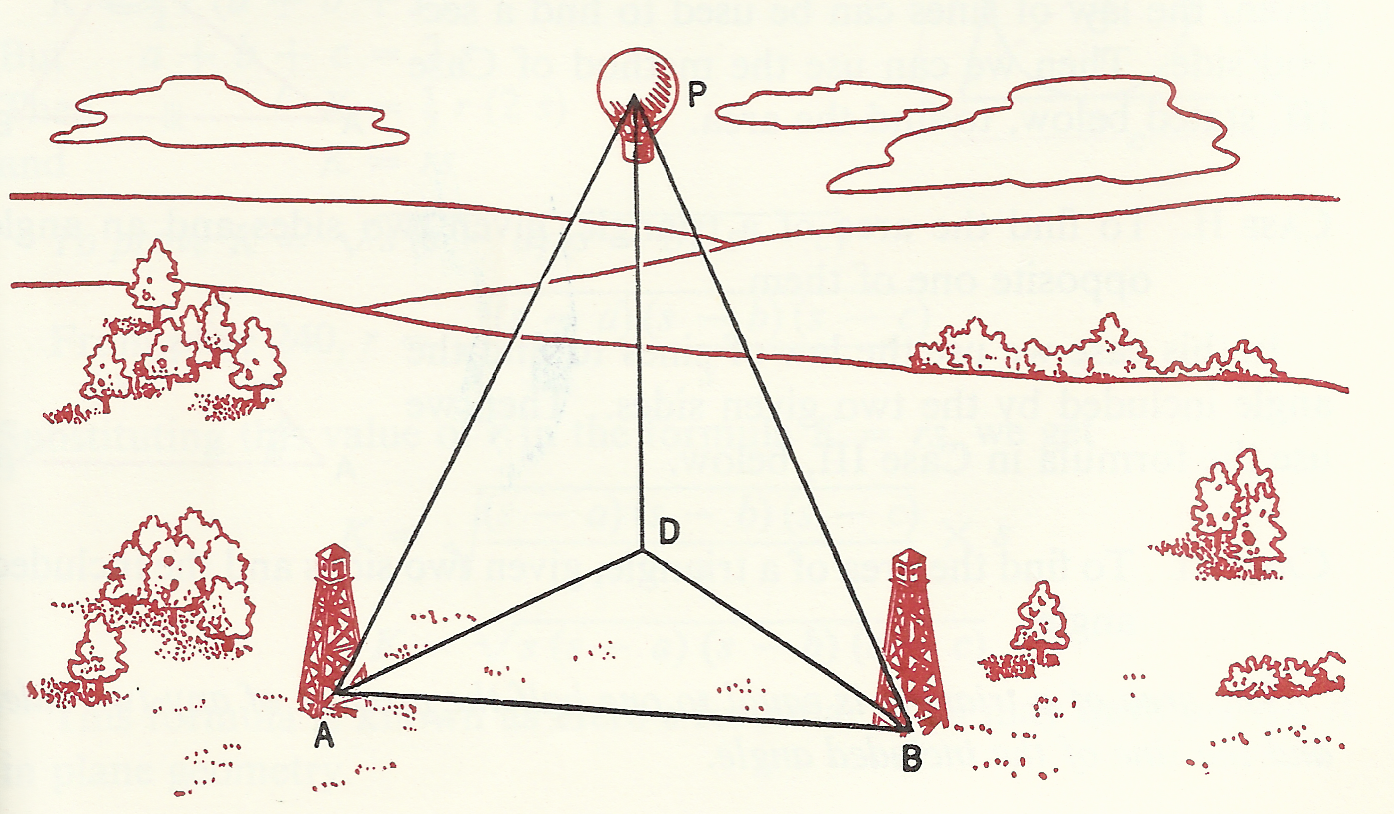
\includegraphics[scale=1]{./oblique-03.png}
  \end{figure}
\end{frame}

\begin{frame}
  \frametitle{End of Lesson}
Next Lesson: Trigonometric Equations
\end{frame}

\end{document}
